\thispagestyle{thachthuctoanhocnone}
\pagestyle{thachthuctoanhoc}
\everymath{\color{thachthuctoanhoc}}
\graphicspath{{../thachthuctoanhoc/pic/}}
\begingroup
\AddToShipoutPicture*{\put(0,616){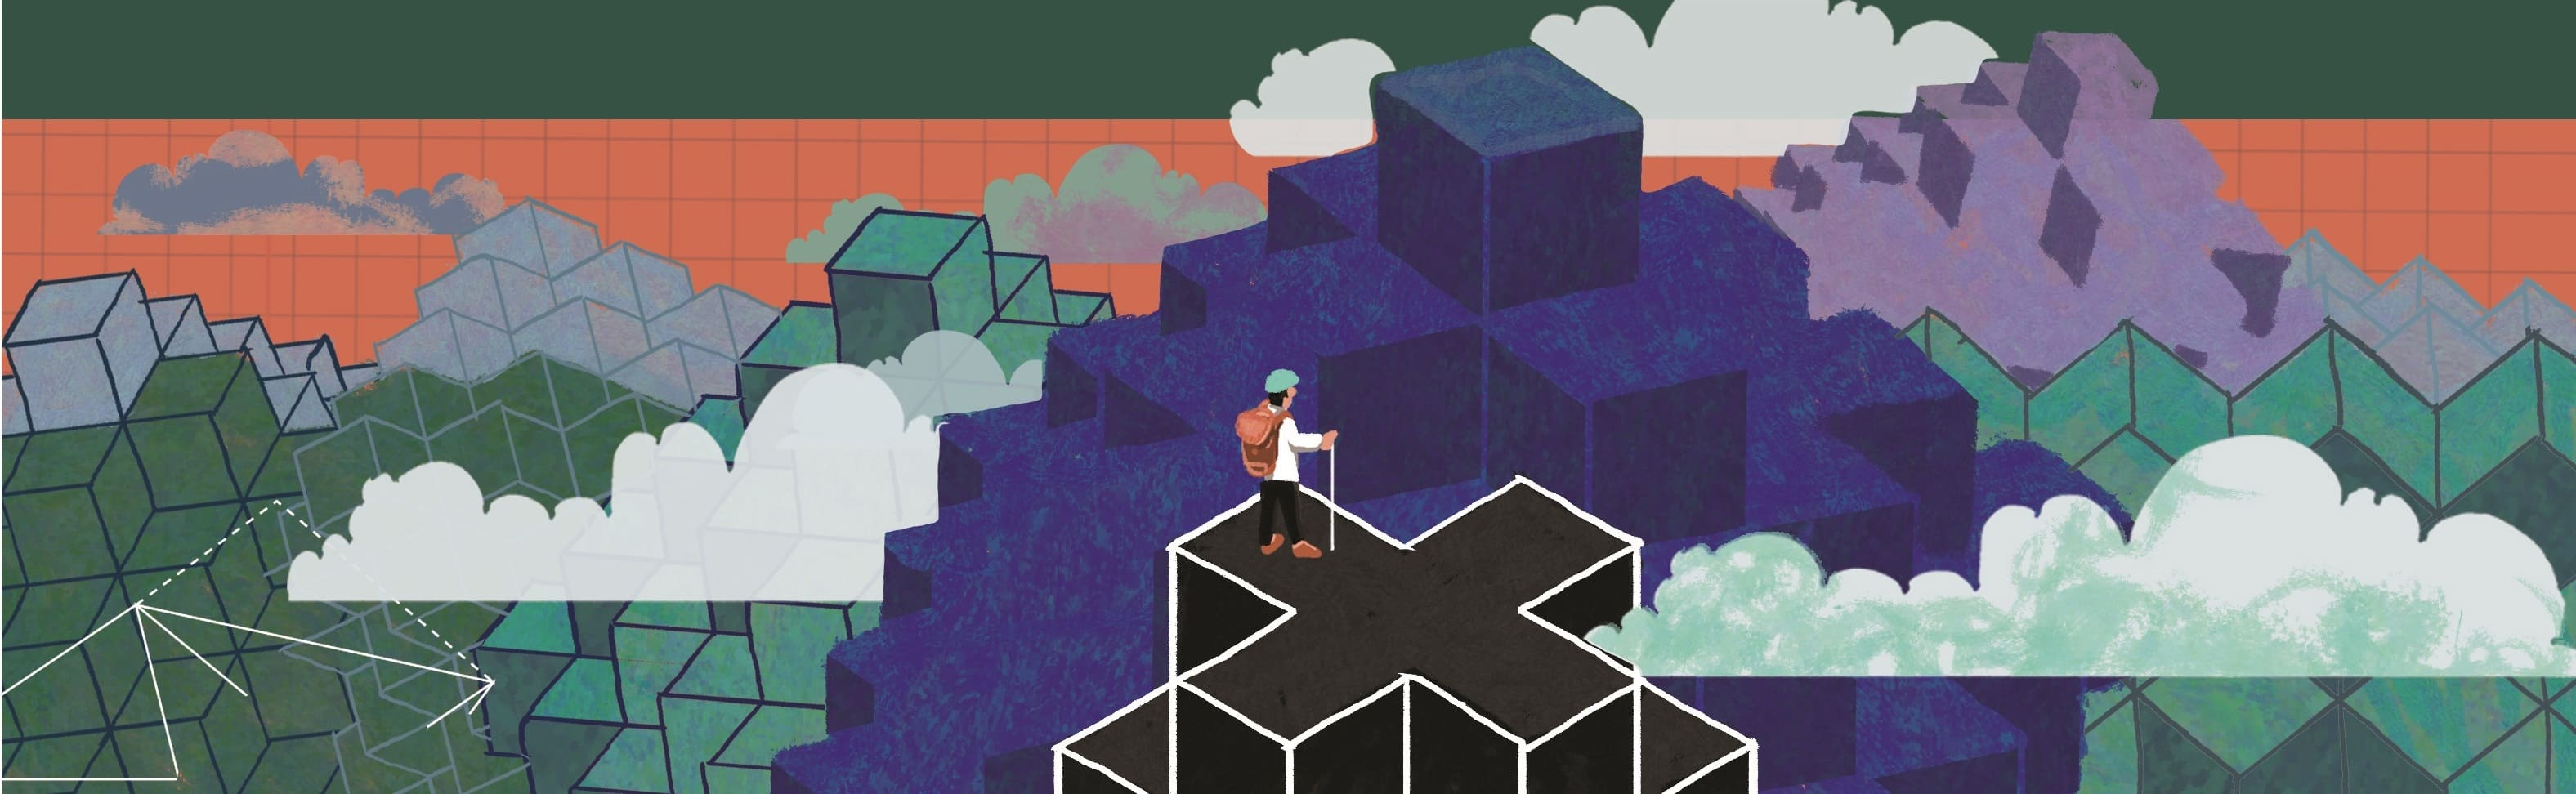
\includegraphics[width=19.3cm]{../thachthuctoanhoc/bannerthachthuc}}}
\centering
\vspace*{4cm}
\endgroup
\vspace*{-8pt}
\begin{tBox}
	\begin{itemize}[leftmargin = 13pt, itemsep = 1.0pt] 
		\item Mỗi bài toán đề xuất (kèm theo lời giải) cần được nêu rõ là bài sáng tác hay bài sưu tầm.
		%		\item Mỗi bài toán đề xuất (kèm theo lời giải) cần được nêu rõ là bài sáng tác hay bài sưu tầm (nếu là bài sưu tầm, cần ghi rõ nguồn).
		\item Bài giải cho mỗi bài toán cần được trình bày trong một file riêng hoặc
		một tờ giấy riêng.
		\item  Người đề xuất bài toán hoặc gửi bài giải cho các bài toán trong mục ``Thách thức kỳ này" cần ghi rõ họ, đệm, tên và nơi làm việc/học tập, số điện thoại liên hệ. Nếu là học sinh (hoặc sinh viên) cần ghi rõ là học sinh lớp mấy (hoặc sinh viên năm thứ mấy).
		\item Các bài toán trong mục Thách thức kỳ này hướng tới các độc giả là học sinh phổ thông; được phân chia thành các mức độ $B$, $A$, và được sắp xếp theo độ khó tăng dần, theo đánh giá chủ quan của Ban biên tập. Các bài toán mức độ $B$ không đòi hỏi các kiến thức vượt quá chương trình môn Toán cấp THCS; các bài toán mức độ $A$ không đòi hỏi các kiến thức vượt quá chương trình môn Toán cấp THPT.
		\item Cách thức gửi bài toán đề xuất hoặc lời giải: gửi file thu được bằng cách scan, ảnh chụp (rõ nét) của bản viết tay, hoặc được soạn thảo bằng các phần mềm Latex, Word tới \url{bbt@pi.edu.vn} hoặc gửi qua đường bưu điện tới Tòa soạn (xem địa chỉ tại bìa $2$).
		\item Hạn gửi lời giải cho các bài toán P$731$--P$740$: trước ngày $15/10/2023$.
	\end{itemize}
\end{tBox}
\begin{center}
	\vspace*{-5pt}
	\textbf{\color{thachthuctoanhoc}\color{thachthuctoanhoc}\color{thachthuctoanhoc}THÁCH THỨC KỲ NÀY}
	\vspace*{-5pt}
\end{center}
\begin{multicols}{2}
	\setlength{\abovedisplayskip}{4pt}
	\setlength{\belowdisplayskip}{4pt}
	{\color{thachthuctoanhoc}{\usefont{T5}{qag}{b}{n} P731.}}
	(Mức $B$) Ghép $9$ hình vuông thành một hình chữ nhật như ở hình dưới đây. Biết rằng, hình vuông màu đen có cạnh bằng $1$. Tìm chiều dài và chiều rộng của hình chữ nhật.
	\begin{figure}[H]
		\vspace*{-5pt}
		\centering
		\captionsetup{labelformat= empty, justification=centering}
		\begin{tikzpicture}[thachthuctoanhoc,scale=0.15]
				\draw[fill=black] (0,0) rectangle (1,1);
				\draw  (0.,-9.)-- (9.,-9.);
				\draw  (9.,-9.)-- (9.,0.);
				\draw  (9.,0.)-- (0.,0.);
				\draw  (0.,0.)-- (0.,-9.);
				\draw  (1.,0.)-- (9.,0.);
				\draw  (9.,0.)-- (9.,8.);
				\draw  (9.,8.)-- (1.,8.);
				\draw  (1.,8.)-- (1.,0.);
				\draw  (-10.,-9.)-- (0.,-9.);
				\draw  (0.,-9.)-- (0.,1.);
				\draw  (0.,1.)-- (-10.,1.);
				\draw  (-10.,1.)-- (-10.,-9.);
				\draw  (-6.,1.)-- (1.,1.);
				\draw  (1.,1.)-- (1.,8.);
				\draw  (1.,8.)-- (-6.,8.);
				\draw  (-6.,8.)-- (-6.,1.);
				\draw  (-10.,1.)-- (-6.,1.);
				\draw  (-6.,1.)-- (-6.,5.);
				\draw  (-6.,5.)-- (-10.,5.);
				\draw  (-10.,5.)-- (-10.,1.);
				\draw  (-6.,8.)-- (9.,8.);
				\draw  (9.,8.)-- (9.,23.);
				\draw  (9.,23.)-- (-6.,23.);
				\draw  (-6.,23.)-- (-6.,8.);
				\draw  (-24.,-9.)-- (-10.,-9.);
				\draw  (-10.,-9.)-- (-10.,5.);
				\draw  (-10.,5.)-- (-24.,5.);
				\draw  (-24.,5.)-- (-24.,-9.);
				\draw  (-24.,5.)-- (-6.,5.);
				\draw  (-6.,5.)-- (-6.,23.);
				\draw  (-6.,23.)-- (-24.,23.);
				\draw  (-24.,23.)-- (-24.,5.);	
		\end{tikzpicture}
		\vspace*{-10pt}
	\end{figure} 
	\begin{flushright}
		\textit{Bùi Văn Biên, France (st)}
	\end{flushright}
	{\color{thachthuctoanhoc}{\usefont{T5}{qag}{b}{n} P732.}}
	(Mức $B$) Xét $4$ số thực (không nhất thiết đôi một khác nhau), mà mỗi số có trị tuyệt đối không vượt quá $\dfrac12$, và tổng của ba số bất kỳ, trong bốn số đó, là một số nguyên. Tìm tất cả các giá trị có thể của tổng bốn số đó.
	\begin{flushright}
		\textit{Nguyễn Đức Tấn, Tp. Hồ Chí Minh (st)}
	\end{flushright}
	{\color{thachthuctoanhoc}{\usefont{T5}{qag}{b}{n} P733.}}
	(Mức $B$) Tìm giá trị nhỏ nhất của biểu thức
	\begin{align*}
		S=\left[\dfrac{b+c}a\right]+\left[\dfrac{c+a}b\right]+\left[\dfrac{a+b}c\right]
	\end{align*}
	trong đó $a,b,c$ là các số nguyên dương.
	\begin{flushright}
		\textit{Nguyễn Việt Hùng, Hà Nội}
	\end{flushright}
	
	{\color{thachthuctoanhoc}{\usefont{T5}{qag}{b}{n} P734.}}
	(Mức $B$) Cho hình vuông $ABCD$. Gọi $E$ là trung điểm của $AD$; $H$ là hình chiếu vuông góc của $B$ trên $CE$. Trên đường chéo $AC$, lấy điểm $M$ sao cho $AM=\frac38AC$. Chứng minh rằng, $ME$ song song với $DH$.  
	\begin{center}
		\definecolor{ffvvqq}{rgb}{1,0.3333333333333333,0}
		\definecolor{qqzzcc}{rgb}{0,0.6,0.8}
		\definecolor{qqqqff}{rgb}{0,0,1}
		\definecolor{qqqqffa}{rgb}{1,1,1}
		\begin{tikzpicture}[thachthuctoanhoc,scale=0.75]
			\draw [color=qqzzcc] (-3.3,3.3)-- (2.7,3.3);
			\draw [color=qqzzcc] (-3.3,3.3)-- (-3.3,-2.7);
			\draw [color=qqzzcc] (-3.3,-2.7)-- (2.7,-2.7);
			\draw [color=qqzzcc] (2.7,-2.7)-- (2.7,3.3);
			\draw  (-3.3,0.3)-- (2.7,-2.7);
			\draw  (0.3,-1.5)-- (2.7,3.3);
			\draw  (-3.3,-2.7)-- (0.3,-1.5);
			\draw [color=ffvvqq] (-3.3,3.3)-- (2.7,-2.7);
			\draw  (-3.3,0.3)-- (-1.05,1.05);
			\draw [fill=white] (-3.3,3.3) circle (1.6pt);
			\draw (-3.44,3.79) node {$A$};
			\draw [fill=white] (2.7,3.3) circle (1.6pt);
			\draw (2.72,3.71) node {$B$};
			\draw [fill=white] (2.7,-2.7) circle (1.6pt);
			\draw (2.68,-3.05) node {$C$};
			\draw [fill=white] (-3.3,-2.7) circle (1.6pt);
			\draw (-3.36,-3.09) node {$D$};
			\draw [fill=white] (-3.3,0.3) circle (1.6pt);
			\draw (-3.76,0.47) node {$E$};
			\draw [fill=white] (0.3,-1.5) circle (1.6pt);
			\draw (0.3,-1.85) node {$H$};
			\draw [fill=white] (-1.05,1.05) circle (1.6pt);
			\draw (-0.76,1.49) node {$M$};
		\end{tikzpicture}
	\end{center}
	\begin{flushright}
		\textit{Huỳnh Thanh Hưng, Phú Yên}
	\end{flushright}
	{\color{thachthuctoanhoc}{\usefont{T5}{qag}{b}{n} P735.}}
	(Mức $B$) Tìm tất cả các số nguyên dương $n$, để $n!+n$ là một luỹ thừa với số mũ nguyên dương của một số nguyên tố.
	\begin{flushright}
		\textit{Hà Duy Hưng, Hà Nội}
	\end{flushright}
	{\color{thachthuctoanhoc}{\usefont{T5}{qag}{b}{n} P736.}}
	(Mức $B$) Bạn An có $8$ quả cân có tổng trọng lượng là $16$ kg và trọng lượng mỗi quả, theo đơn vị kg, là một số nguyên dương không vượt quá $8$. Chứng minh rằng, có thể chia $8$ quả cân này thành hai nhóm sao cho các tổng trọng lượng của các quả cân cùng nhóm bằng nhau.
	\begin{flushright}
		\textit{Tường Thanh, Nghệ An}
	\end{flushright}
	{\color{thachthuctoanhoc}{\usefont{T5}{qag}{b}{n} P737.}}
	(Mức $A$) Xét các số thực dương $a,b,c$,  thoả mãn $a^2+b^2+c^2=1$. Tìm giá trị nhỏ nhất của biểu thức
	\begin{align*}
		S=2\left(a^3+b^3+c^3\right)-\left(a+b+c\right).
	\end{align*}
	\begin{flushright}
		\textit{Kiều Đình Minh, Phú Thọ}
	\end{flushright}
	{\color{thachthuctoanhoc}{\usefont{T5}{qag}{b}{n} P738.}}
	(Mức $A$) Cho tam giác $ABC$ ngoại tiếp đường tròn $(I)$. Gọi $J$ là tâm đường tròn bàng tiếp góc $A$ của tam giác đó. Trên cạnh $BC$, lấy điểm $D$ tùy ý, sao cho ba điểm $A,I,D$ không thẳng hàng. Đường thẳng $AD$ cắt các đường thẳng $IB, IC$, tương ứng, tại $E,F$. Gọi $H$ là trực tâm của tam giác $IEF$, và gọi $K$ là trung điểm của $AD$. Chứng minh ba điểm $K, H, J$ thẳng hàng.
	\begin{center}
		\definecolor{ffvvqq}{rgb}{1,0.3333333333333333,0}
		\definecolor{qqzzcc}{rgb}{0,0.6,0.8}
		\definecolor{qqqqff}{rgb}{0,0,1}
		\definecolor{qqqqffa}{rgb}{1,1,1}
		\definecolor{cqcqcq}{rgb}{0.7529411764705882,0.7529411764705882,0.7529411764705882}
		\begin{tikzpicture}[thachthuctoanhoc,scale=0.45]
			\draw [color=qqzzcc] (-3.679901022761026,4.943589529660562)-- (-4.58,-1.6);
			\draw [color=qqzzcc] (-4.58,-1.6)-- (3.08,-1.6);
			\draw [color=qqzzcc] (3.08,-1.6)-- (-3.679901022761026,4.943589529660562);
			\draw [color=ffvvqq] (-3.257494355051633,-1.6)-- (-3.679901022761026,4.943589529660562);
			\draw [color=ffvvqq] (-4.58,-1.6)-- (-2.151513063456181,0.5173053476685014);
			\draw [color=ffvvqq] (-3.4275087350979017,1.0337281160719551)-- (3.08,-1.6);
			\draw [dashed] (-3.4686976889063295,1.671794764830281)-- (0.6515130634561829,-7.600391557576506);
			\draw  (-2.151513063456181,0.5173053476685014) circle (2.117305347668501cm);
			\draw  (0.6515130634561829,-7.600391557576506) circle (6.000391557576506cm);
			\draw [color=qqzzcc] (-4.58,-1.6)-- (-5.292904303746716,-6.782711296880436);
			\draw [color=qqzzcc] (3.08,-1.6)-- (4.824890183355734,-3.2890550757724784);
			\draw [fill=white] (-3.679901022761026,4.943589529660562) circle (2.5pt);
			\draw (-3.7075216945790075,5.430778676473025) node {$A$};
			\draw [fill=white] (-4.58,-1.6) circle (2.5pt);
			\draw (-5.171417300932007,-1.6163200271099578) node {$B$};
			\draw [fill=white] (3.08,-1.6) circle (2.5pt);
			\draw (3.5014736499140704,-1.2848719652941842) node {$C$};
			\draw [fill=white] (-2.151513063456181,0.5173053476685014) circle (2.5pt);
			\draw (-1.9397986982282145,0.012402451962288) node {$I$};
			\draw [fill=white] (0.6515130634561829,-7.600391557576506) circle (2.5pt);
			\draw (0.6565444526620129,-8.41453873427639) node {$J$};
			\draw [fill=white] (-3.257494355051633,-1.6) circle (2.5pt);
			\draw (-3.3484529609452527,-2.058250776197656) node {$D$};
			\draw [fill=white] (-3.4686976889063295,1.671794764830281) circle (2.5pt);
			\draw (-2.80379702736733282,1.9124706683174956) node {$K$};
			\draw [fill=white] (-3.327960493319134,-0.5083943985466047) circle (2.5pt);
			\draw (-2.84462557094746,-0.667344980266746) node {$E$};
			\draw [fill=white] (-3.4275087350979017,1.0337281160719551) circle (2.5pt);
			\draw (-3.818004381850932,0.9800231237802691) node {$F$};
			\draw [fill=white] (-2.9332617149580074,0.4668413261447786) circle (2.5pt);
			\draw (-2.685556837313705,0.8842990928723823) node {$H$};
			\draw [fill=white] (0.6515130634561829,-1.6) circle (2.5pt);
			\draw [fill=white] (-5.292904303746716,-6.782711296880436) circle (2.5pt);
			\draw [fill=white] (4.824890183355734,-3.2890550757724784) circle (2.5pt);
		\end{tikzpicture}
	\end{center}
	\begin{flushright}
		\textit{Lưu Công Đông, Hà Nội}
	\end{flushright}
	{\color{thachthuctoanhoc}{\usefont{T5}{qag}{b}{n} P739.}}
	(Mức $A$) Cho dãy số $(a_n)$, xác định bởi
	\begin{align*}
		a_n=\left[\dfrac n{\sqrt2}\right]+\left[\dfrac n{\sqrt3}\right],\quad\text{với mọi $n\in\mathbb N^*$}.
	\end{align*}
	Chứng minh rằng, trong dãy $(a_n)$ chứa vô hạn số chẵn và vô hạn số lẻ.
	\begin{flushright}
		\textit{Nguyễn Tiến Lâm, Hà Nội}
	\end{flushright}
	{\color{thachthuctoanhoc}{\usefont{T5}{qag}{b}{n} P740.}}
	(Mức $A$) Cho bảng ô vuông kích thước $2023\times 2023$. Tìm số nguyên dương $n$ nhỏ nhất, sao cho có thể đặt $n$ viên bi vào các ô vuông con của bảng, đảm bảo các điều kiện sau được đồng thời thoả mãn:
	\vskip 0.1cm
	$i/$ Ở mỗi ô vuông con chỉ có tối đa một viên bi;
	\vskip 0.1cm
	$ii/$ Với mỗi ô vuông con không có bi, tổng số viên bi ở hàng và cột chứa ô đó không nhỏ hơn $2023$.
	\begin{flushright}
		\textit{Tô Trung Hiếu, Nghệ An (st)}
	\end{flushright}
\end{multicols}
%\newpage
%\centerline{{\large{\textbf{\color{thachthuctoanhoc}GIẢI BÀI KỲ TRƯỚC}}}}
%\vspace*{-5pt}
%\begin{multicols}{2}
%\end{multicols}	